%#########################################################
\chapter{Diffusion Modeling to Study Microarchitecture in Human Skeletal Muscles}
\label{ch: DiffusionExp}
%#########################################################
The resolution of the MR images is not sufficient to perform direct measurements of the muscle fiber geometry and other physical parameters such as membrane permeability at the level of individual fiber. 
While typical resolution of the MR images is $\approx \SI{e-3}{\m}$ histology studies showed that cross-sectional liner dimensions are in the range of $10^{-5} - \SI{e-4}{\m}$ \cite{TAYLOR200335}. 
In recent years a number of diffusion models were developed in the effort to relate macroscopic signal measured in MRI experiments to the microscopic parameters of muscle tissue. 
%-new paragraph-%

%-new paragraph-%
This chapter presents work on application of two diffusion models to interpret disuse atrophy and age related changes in human lower leg muscle.

%=========================================================
\section{Monitoring Changes in the Medial Gastrocnemius in Disuse Atrophy Induced by Unilateral Limb Suspension}
\label{sec: DTI ULLS}
%=========================================================
The feasibility of diffusion tensor imaging (DTI) of skeletal muscle including muscle fiber tracking for extraction of fiber lengths and pennation angles has been established, and the technique has been applied to monitor muscle injury, aging, gender related differences, and compartmental syndrome~\cite{RND1, RND2, RND3, RND4, RND5, RND6}. 
Additionally, some studies have explored changes in muscle DTI with atrophy; e.g., arising from age-related atrophy in human skeletal muscle~\cite{RND7}, from denervation and from Achilles tenotomy-induced atrophy in rodent models~\cite{RND8, RND9}.
Further, DTI combined with diffusion models is increasingly being used to explore tissue microstructural parameters such as fiber diameter, permeability or intracellular volume fraction~\cite{RND10}.
While most modeling studies have focused on the brain, a few recent studies have extended modeling efforts to the diffusion in skeletal muscle~\cite{RND11, RND12, RND13}. 
Recent studies have combined combine magnetic resonance imaging deformation analyses and diffusion tensor imaging tractography in the medial gastrocnemius~\cite{RNSS4,RNCS4}. 
Karakuzu~et~al. showed that submaximal plantar flexion activity at 15\% Maximum voluntary contraction (MVIC) causes heterogeneous length changes along the fascicles of human medial gastrocnemius (MG) muscle~\cite{RNCS4}.
The heterogeneity of fascicle strains was explained on the basis of epimuscular myofascial force transmission. 
%-new paragraph-%

%-new paragraph-%
It is well established that disuse (e.g., by chronic unloading) leads to skeletal muscle atrophy that is accompanied by a significant loss of muscle force~\cite{RNS1}.
The Unilateral Limb Suspension (ULLS) is a validated model to study the effects of chronic unloading~\cite{RNS8}.
Unilateral limb suspension results in both loss of muscle mass (muscle fiber atrophy) as well as a decrease in muscle force~\cite{RNS8}.
Prior studies of induced immobilization indicate that muscle remodeling with inactivity is a fast process that occurs after about a week of unloading~\cite{RNS8, RNS5}.
These studies documented the decrease in both fiber length and pennation angle, a decrease in Focal Adhesion Kinase content ($-20\%$) and activity ($-30\%$), associated with a $50\%$ fall in muscle protein synthesis and a $5\%$ decrease in quadriceps muscle anatomical cross-sectional area (ACSA)~\cite{RNS8, RNS5}.
DTI with its ability to probe at the microstructural level is ideally suited to investigate potential muscle remodeling that occurs with chronic unloading.
However, no studies to date have investigated unloading induced changes in skeletal muscle using DTI in human subjects.
%~~~~~~~~~~~~~~~~~~~~~~~~~~~~~~~~~~~~~~~~~~~~~~~~~~~~~~~~~
\subsection{Methods}
%~~~~~~~~~~~~~~~~~~~~~~~~~~~~~~~~~~~~~~~~~~~~~~~~~~~~~~~~~
%---------------------------------------------------------
\subsubsection{\textit{In-vivo} experiments}
%---------------------------------------------------------
The study was carried out under the approval of the Medical Research Ethics Board of UC~San~Diego and conformed to all standards for the use of human subjects in research as outlined in the Declaration of Helsinki on the use of human subjects in research.
IRB approval was obtained from the Medical Research Ethics Board of UC~San~Diego and all subjects were recruited after obtaining written informed consent. A total of 7 normal healthy young subjects (2 females, $29.1 \pm 5.7$ years, body mass $75.4 \pm \SI{22.7}{\kilogram}$, height $168.1 \pm \SI{7.4}{\centi\meter}$) were recruited for this study.
The criterion for inclusion was that subjects should be moderately physically active. Subjects participating in competitive sports as well as those with any surgical procedures performed on the lower leg were excluded.
%---------------------------------------------------------
\subsubsection{Study design} 
%---------------------------------------------------------
The effect of chronic unloading on the force production capability and diffusion tensor indices of the MG muscle were assessed by comparing the baseline (pre) to immediately after four weeks of limb suspension (post).
During the four week suspension period, subject compliance to the protocol was monitored at two weeks to check for muscle atrophy (MRI morphological scan) and loss of force production.
In addition, compliance was also monitored by a wireless activity tracker that was integrated into the crutches; the subject was not informed of the tracker to ensure that it was not removed or tampered with to simulate crutch usage.
After the four week suspension, subjects were required to attend structured physical rehabilitation sessions.
MRI morphological scans were performed at the end of the rehabilitation period (four weeks) to confirm that the muscle had recovered to baseline status.
%---------------------------------------------------------
\subsubsection{Unilateral Limb Suspension (ULLS)}
%---------------------------------------------------------
The ULLS model is an established model of inducing controlled atrophy~\cite{RNS19} and was used in the current study to induce muscle atrophy on the non-dominant leg with four weeks of chronic unloading.
The dominant leg was self-identified by subjects as the one they preferentially used to regain balance from a jostle.
The non-dominant leg was the left leg for all subjects in this study.
The ULLS protocol allowed the subjects a reasonable amount of freedom to carry out their daily activities including driving since the dominant leg (right in this study) was not unloaded.
A crutch was used to prevent the foot (of the left leg) from touching the ground.
The right foot was raised with a $\SI{5}{\centi\meter}$ sole on the shoe to further minimize accidental loading of the foot.
%---------------------------------------------------------
\subsubsection{MR imaging} 
%---------------------------------------------------------
Subjects were positioned supine in a $\SI{3}{\tesla}$ whole-body scanner (GE Medical Systems, WI, USA) and only the limb selected for suspension was scanned (pre- and post-suspension).
A custom-built receive-only phased array coil with a large FOV was used to image approximately $\SI{30}{\centi\meter}$ of the lower leg without moving the subject or coil; the intent was to cover the medial gastrocnemius muscle from its origin to insertion in two acquisitions without having to reposition the subject in the coil.
The coil moved relative to the magnet between acquisitions, the subject did not move with respect to the coil.
One anatomical slice was common between the two sets of acquisitions and the two sets were reoriented by a transformation obtained from the rigid alignment of the slice common to both sets.
The subject's leg was fully extended while the foot was maintained in a fixed position at $\approx \SI{15}{\degree}$ in plantarflexion; the foot rested on an adjustable wedge to maintain the angle constant for the scan duration. This foot position was used to ensure that there was no passive tension in the lower leg muscles.
%-new paragraph-%

%-new paragraph-%
The MRI pulse sequence used in the image acquisition was a fat suppressed single shot EPI spin-echo sequence with monopolar diffusion gradients (diffusion gradient duration, $\delta = \SI{12}{\milli\second}$, and diffusion time $\Delta = \SI{20}{\milli\second}$). 
Spectral-spatial water selective excitation was used to suppress fat.
The total number of slices (acquired in two multi-slice 2D sets) required to cover the calf muscles ranged from 32 to 40 slices.
$B_0$ shimming in the selected region of interest was performed with vendor supplied automated second order shims.
Thirty-two non-collinear gradient directions with a \mbox{\textit{b-}value} of $\SI{400}{\second \per \milli\meter^2}$ were used to map the direction dependent diffusion.
Imaging parameters: echo time (TE) $\SI{52.7}{\milli\second}$, repetition time (TR) $\SI{7000}{\milli\second}$ ms with 4 signal averages, field of view (FOV) $240 \times 240 \; \SI{}{\milli\meter^2}$, slice thickness $\SI{5}{\milli\meter}$, no gap and acquisition matrix $80 \times 80$; no parallel imaging was employed. The $80 \times 80$ matrix was reconstructed to $128 \times 128$ matrix by partial fourier with homodyne reconstruction.
The homodyne algorithm pre-weights the \mbox{\textit{k-}space} data so that when the real part of the image is extracted, it corresponds to uniform weighting in \mbox{\textit{k-}space}~\cite{RND20}.
The $128 \times 128$ matrix is then extrapolated to a $256 \times 256$ matrix yielding a voxel resolution of $\SI{0.94}{\milli\meter} \times \SI{0.94}{\milli\meter} \times \SI{5.00}{\milli\meter}$.
In addition to the diffusion weighted images, a morphological volume was acquired with a fat saturated fast gradient echo (FGRE) sequence for two echo times with the following parameters: $\mathrm{TE_1}/\mathrm{TE_2}$/TR: $\SI{3.2}{\milli\second}/\SI{5.6}{\milli\second}/\SI{350}{\milli\second}$ and a flip angle (FA) of $\SI{20}{\degree}$; all geometric parameters were the same as in the DTI scans.
The acquired morphological volume was used to generate phase maps to correct $B_0$ distortions in the echo planar images.
The total scan time including the morphological images for each session was 17 minutes. 
%---------------------------------------------------------
\subsubsection{Force measurements}
%---------------------------------------------------------
Isometric MVIC of the plantarflexor muscles was determined for each subject prior to MR imaging. For this purpose, the ankle was fixed in a neutral position ($\SI{90}{\degree}$ angle between the axis of the foot and the shank).
To estimate the maximum force acting along the Triceps Surae tendon, the force recorded by the force transducer was divided by the Achilles tendon moment arm corresponding to $\SI{90}{\degree}$ angle between the axis of the foot and the shank detailed earlier~\cite{RNS20}.
In brief, a sagittal MR image of the lower leg and foot was used to identify the joint (ankle) center of rotation as well as Achilles tendon line of action (the latter marked as a straight line along the center of the tendon). 
The perpendicular distance of the joint center to the line of action was measured as the Achilles tendon moment arm~\cite{RNS20}.
The measured muscle force is that generated by the gastrocnemius (lateral and medial) and the soleus muscles.
%---------------------------------------------------------
\subsubsection{Muscle volume measurements}
%---------------------------------------------------------
The manual contouring was performed using parametric Bezier curves every fifth slice using OsiriX~\cite{RND22}.
Automated interpolation was performed for the intervening slices; all automated contours were examined and edited if needed.
%---------------------------------------------------------
\subsubsection{Image preprocessing and DTI indices computation}
%---------------------------------------------------------
Figure~\ref{fig: DTI-flowchart} is the flowchart of the sequence of image processing steps.
All diffusion weighted image volumes were registered to the baseline ($b=0$) image to correct for eddy currents and motion related artifacts using the \textit{eddy} algorithm from FSL~\cite{RND23}. 
The phase images of the dual echo (FGRE) volumes were used to correct for $B_0$ field inhomogeneities using the \textit{fugue} algorithm from FSL~\cite{RND23}.
Diffusion weighted images were then denoised using a Joint Rician Linear Minimum Mean Square Error (LMMSE) estimator~\cite{RND24}. 
The noise in magnitude MR images is best modeled by a Rician distribution and the LMMSE estimator has been shown to out-perform other Rician denoising techniques~\cite{RND25}.
The tensor was calculated from the distortion corrected and denoised data using a Gaussian model of diffusion.
The tensor was then diagonalized to yield the eigenvalues followed by the calculation of the fractional anisotropy (FA), apparent diffusion coefficient (ADC) and coefficient of planarity (CP) maps. 
The contour of the MG traced in the FGRE volume slices was transferred to the DTI indices map.
Average values of the DTI indices were obtained from a $5 \times 5$ region of interest (ROI) automatically placed at the centroid of the MG mask at each anatomical slice (in most subjects, 40 axial slices were required to cover the MG); this placement ensured that the ROI was not at the edges which would bias estimates due to partial volume effects. 
A manual check was also made to ensure that the ROI was not in the region of a blood vessel, fascia or contained artifacts; such ROIs were moved manually to avoid artifacts. 
Though the ROI was small at 25 pixels/slice, the total number of pixels across all slices was $\approx 900 (25 \times 36)$ ensuring the robustness of the DTI indices. 
%*********************************************************
\begin{figure}[!htb]
\vspace{+0.2cm}
\centering
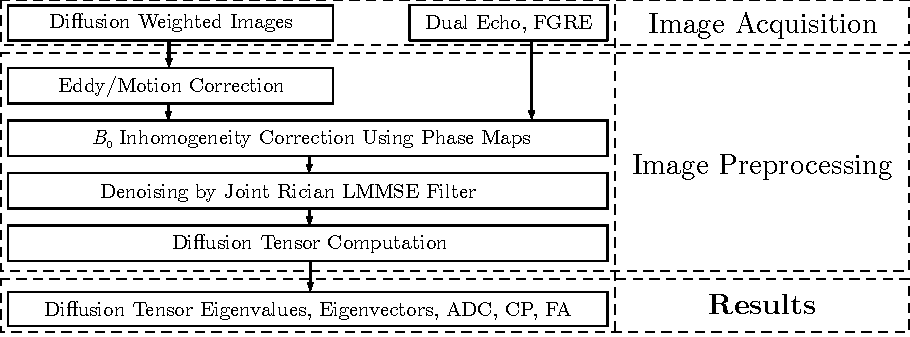
\includegraphics[width=0.9\textwidth]{Figures/DTI_flowchart.pdf}
\caption[The image processing flowchart showing the sequence of steps leading to the extraction of the diffusion tensor indices]{The image processing flowchart showing the sequence of steps leading to the extraction of the diffusion tensor indices.}
\label{fig: DTI-flowchart}
\end{figure}
%*********************************************************
%---------------------------------------------------------
\subsubsection{Simulation}
%---------------------------------------------------------
The model used here closely follows that proposed originally by Karampinos~et~al.~\cite{RND12}. 
Simulations were carried out by varying the fit parameters ($\alpha$, $d$, $\tau_{\mathrm{in}}$, $\nu_{\mathrm{in}}$, $\nu_{\mathrm{col}}$) to compute DTI eigenvalues. 
The five parameter-space was searched to find the optimal combination of the five parameters that minimized the normalized root mean square difference (NRMSE) between the eigenvalues computed from the simulation and those determined from experiments (Equation~\ref{eq: KargerRMSE}).
%.........................................................
\begin{equation}\label{eq: KargerRMSE}
\mathrm{NRMSE} = \sqrt{\dfrac{\sum\limits_{i=1}^3 \left( \lambda_{i,\mathrm{expr}}-\lambda_{i, \mathrm{sim}} \right)^2}{\sum\limits_{i=1}^3 \lambda_{i,\mathrm{expr}}^2}}
\end{equation}
%.........................................................
where $\lambda_{i,\mathrm{expr}}$ is the experimentally determined eigenvalues while $\lambda_{i,\mathrm{sim}}$ is the eigenvalue from the model simulation. 
Since there are five variables that are fit to the model, the search space was limited to physiologically relevant ranges in order to prevent the search from minimizing at non-physiological values, these ranges were taken from~\cite{RND12}. 
The simulations were carried out with the values for intra-cellular diffusion coefficient ($D_{\mathrm{in}}$), extracellular matrix diffusion coefficient ($D_{\mathrm{ex}}$), intra-cellular $\mathrm{T_2}$ ($\mathrm{T}_{\mathrm{2,in}}$), and extra-cellular $\mathrm{T_2}$ ($\mathrm{T}_{\mathrm{2,ex}}$) taken from the literature~\cite{RND12, RND26}.
It should be noted here that Karampinos~et~al. fitted $D_{\mathrm{in}}$ and $D_{\mathrm{ex}}$ to the diffusion model, but these variables were kept fixed in the current paper at the values obtained for young normal subjects in the former paper~\cite{RND12}. 
This was done to limit the number of model variables in order to increase the robustness of the fit.
Further, as $D_{\mathrm{in}}$ is determined by the various intracellular membrane and protein structure; it is not anticipated to change with atrophy. 
$D_{\mathrm{ex}}$, the diffusion in the extracellular compartment is determined by the collagen fraction in the endomysium and the diffusion coefficient of water.
Based on the findings from imaging that \% connective tissue fraction does not change with atrophy (unreported study on the same subjects), it is also anticipated that \% collagen fraction in the endomysium may not change significantly with atrophy. 
The experimental values of the eigenvalues ($\lambda_{i,\mathrm{expr}}$) used in obtaining the optimal solution from the simulation were the mean values of all the subjects for pre- and post-suspension. 
The optimization was performed in Wolfram Research, Inc., Mathematica, (Version 11.3, Champaign, IL). 
The conjugate gradient search algorithm was used to find the parameters that minimize NRMSE. 
As this method only guarantees a local minimum, the global minimum was obtained by a search performed over all combinations of the five-parameter space; the range and step size of the search space are provided in Table~\ref{tab: Karger2}.
%=========================================================
\begin{table}[!htb]
\vspace{+0.2cm}
\caption[Tissue microstructural parameters from bicompartmental diffusion model]{Tissue microstructural parameters from bicompartmental diffusion model.}
\label{tab: Karger2}
\begin{center}
\begin{tabular}{@{}llllll@{}}
\toprule[1pt]\midrule[0.3pt]
  & & Pre-ULLS & Post-ULLS & Range     & Step size \\ \midrule
$\alpha$     & & 0.55     & 0.95      & 0.05 - 0.95 & 0.05      \\[6pt]
$d$ & $[\SI{}{\micro\meter}]$   & 82       & 65        & 50 - 110    & 5         \\[6pt]
$\tau_{\mathrm{in}}$ & $\left[\SI{}{\second}\right]$   & 0.8      & 2.6       & 0.8 - 2.6   & 0.2       \\[6pt]
$\nu_{\mathrm{in}}$  & &0.95     & 0.89      & 0.89 - 0.95 & 0.0025    \\[6pt]
$\nu_{\mathrm{col}}$ & &0.5      & 0.6       & 0.5 - 0.6   & 0.0025    \\ \midrule[0.3pt]\toprule[1pt]
\end{tabular}
\end{center}
\vspace{-0.2cm}
\end{table}
%=========================================================
%---------------------------------------------------------
\subsubsection{Statistical analysis} 
%---------------------------------------------------------
The outcome variables of the analysis are the diffusion tensor indices ($\lambda_1$, $\lambda_2$, $\lambda_3$, FA and CP). 
The assumption of normality of data was tested using both the Shapiro-Wilk test and by visual inspection of quantile-quantile plots. 
Since deviations from normality were only minor and no non-parametric alternative to factorial ANOVA exists, differences between pre- and post-ULLS values were assessed using two-way repeated measures ANOVAs. 
Data are reported as mean $\pm$ standard deviation. 
For all tests, the level of significance was set at 0.05. 
The statistical analyses were carried out using SPSS for Mac OSX (SPSS 23.0, IBM Inc, Armonk, NY).
%~~~~~~~~~~~~~~~~~~~~~~~~~~~~~~~~~~~~~~~~~~~~~~~~~~~~~~~~~
\subsection{Bicompartmental Diffusion Model with Exchange}
\label{subsec: bicompart}
%~~~~~~~~~~~~~~~~~~~~~~~~~~~~~~~~~~~~~~~~~~~~~~~~~~~~~~~~~
The multi-compartment diffusion model used here is originally proposed by K\"arger~\cite{KARGER19881} and extended by Karampinos~\cite{RND12}. 
Muscle fibers are approximated with infinite cylinders of an elliptical cross-section and ratio between major axis $\alpha = d_s/d_l$ as shown in Figure~\ref{fig: KargerModel}. 
%*********************************************************
\begin{figure}[!htb]
\vspace{+0.2cm}
\centering
\includegraphics[scale=.3]{Figures/FibersModel.pdf}
\caption[Schematic of muscle fibers and endomaysium matrix]{Schematic of muscle fibers and endomaysium matrix.}
\label{fig: KargerModel}
\end{figure}
%*********************************************************
Muscle fiber diameter $d$ defined as the mean of the short axis and long axis lengths.
The model allows exchange between two compartments: the intracellular space (inside the muscle fiber) and the extracellular space (collagenous intramuscular connective tissue consisting of endomysium and perimysium).
The volumes of the two compartments are denoted as $\nu_{\mathrm{in}}$ (intramyocellular volume fraction) and $\nu_{\mathrm{ex}}$ (extracellular volume fraction), with $\nu_{\mathrm{in}} + \nu_{\mathrm{ex}} = 1$. 
Further, the collagen fraction in the extracellular matrix is represented by $\nu_{\mathrm{coll}}$. 
The last parameter of the fit is the intracellular residence time $(\tau_{\mathrm{in}})$, which is related to the permeability ($\kappa$) of the sarcolemma (i.e. the cell membrane of muscle fibers) through the relationship: $\tau_{\mathrm{in}} = d/2\kappa$. 
Total MR signal $S$ which is a function of time $t$ and \mbox{\textit{b-}value} is a sum of signals from intracellular and extracellular compartments:
%.........................................................
\begin{equation}\label{eq: Karger Signal}
S(t,b) = S_{\mathrm{in}}(t,b)+S_{\mathrm{ex}}(t,b)
\end{equation}
%.........................................................
Time evolution of the signals $S_\mathrm{in}$ and $S_\mathrm{ex}$ can be found from the system of ordinary differential equations:
%.........................................................
\begin{equation}\label{eq: Karger ODE}
{\setstretch{1.0}
\begin{cases}
\dfrac{dS_{\mathrm{in}}}{dt}=-q^2D^{\mathrm{app}}_{\mathrm{in}}S_{\mathrm{in}}-\dfrac{1}{\tau_{\mathrm{in}}}S_{\mathrm{in}}+\dfrac{1}{\tau_{\mathrm{ex}}}S_{\mathrm{ex}}-\dfrac{1}{\mathrm{T}_{2,\mathrm{in}}}S_{\mathrm{in}}\\[20pt]
\dfrac{dS_{\mathrm{ex}}}{dt}=-q^2D^{\mathrm{app}}_{\mathrm{ex}}S_{\mathrm{ex}}-\dfrac{1}{\tau_{\mathrm{ex}}}S_{\mathrm{ex}}+\dfrac{1}{\tau_{\mathrm{in}}}S_{\mathrm{in}}-\dfrac{1}{\mathrm{T}_{2,\mathrm{ex}}}S_{\mathrm{ex}}
\end{cases}
}
\end{equation}
%.........................................................
where $q$ is a product of gyromagnetic ratio $\gamma$, gradient $G$ of duration $\delta$. 
Using $q$ the \mbox{\textit{b-}value} can be expressed as $b=q^2(\Delta-\delta/3)$, $\Delta$ is time separation between diffusion gradients. 
With initial conditions:
%.........................................................
\begin{equation}\label{eq: Karger IC}
{\setstretch{1.0}
\begin{aligned}
& S_{\mathrm{in}}(0,b)=\nu_{\mathrm{in}}\\[10pt]
& S_{\mathrm{ex}}(0,b)=\nu_{\mathrm{ex}}\\[10pt]
& \dfrac{S_{\mathrm{in}}(0,b)}{\tau_{\mathrm{in}}}=\dfrac{S_{\mathrm{ex}}(0,b)}{\tau_{\mathrm{ex}}}
\end{aligned}
}
\end{equation}
%.........................................................
system of Equations~\ref{eq: Karger ODE} has the solution:
%.........................................................
\begin{equation}\label{eq: Karger Solution}
S(t,b)=\nu'_{\mathrm{in}} e^{-q^2tD'_{\mathrm{in}}}+\nu'_{\mathrm{ex}} e^{-q^2tD'_{\mathrm{ex}}}
\end{equation}
%.........................................................
with modified volumes and diffusion coefficients:
%.........................................................
\begin{equation}\label{eq: Karger v modified}
\begin{array}{l}
\nu'_{\mathrm{ex}} = \dfrac{1}{D'_{\mathrm{ex}}-D'_{\mathrm{in}}} \left[\nu_{\mathrm{in}}\left( D^{\mathrm{app}}_{\mathrm{in}} + \dfrac{1}{q^2 \mathrm{T}_{2,\mathrm{in}}} \right) + \nu_{\mathrm{in}}\left( D^{\mathrm{app}}_{\mathrm{in}} + \dfrac{1}{q^2 \mathrm{T}_{2,\mathrm{in}}} \right) - D'_{\mathrm{in}} \right]\\[10pt]
\nu'_{\mathrm{in}} = 1 - \nu'_{\mathrm{ex}}
\end{array}
\end{equation}
%.........................................................
%.........................................................
\begin{equation}\label{eq: Karger ADC}
\begin{split}
D'_\mathrm{in,ex} &= \frac{1}{2}\left( D^{\mathrm{app}}_\mathrm{in} + D^{\mathrm{app}}_\mathrm{ex} + \frac{1}{q^2}\left(\frac{1}{\tau_{\mathrm{in}}} + \frac{1}{\tau_{\mathrm{ex}}} + \frac{1}{\mathrm{T}_{2,\mathrm{in}}} + \frac{1}{\mathrm{T}_{2,\mathrm{ex}}} \right) \right) \mp \\ &\mp \frac{1}{2}\sqrt{\left( D^{\mathrm{app}}_\mathrm{in} - D^{\mathrm{app}}_\mathrm{ex} + \frac{1}{q^2}\left(\frac{1}{\tau_{\mathrm{in}}} - \frac{1}{\tau_{\mathrm{ex}}} - \frac{1}{\mathrm{T}_{2,\mathrm{in}}} + \frac{1}{\mathrm{T}_{2,\mathrm{ex}}} \right) \right) + \frac{4}{q^4\tau_{\mathrm{in}}\tau_{\mathrm{ex}}}}\\
\end{split}
\end{equation}
%.........................................................
\\
Intracellular apparent diffusion coefficient $D^{\mathrm{app}}_\mathrm{in}$ is found by investigating signal attenuation due to diffusion inside two impermeable walls separated by distance $d$ with gradient $G$ applied perpendicular to these walls. 
Signal $S$ defined as ratio between $\bar{M}$ and $M_{0}$ expressed through conditional probability $P(z_2|z_1, \Delta)$:
%.........................................................
\begin{equation}\label{eq: Karger AppEx}
S (t,b)= \dfrac{1}{d}\iint dz_1 dz_2  \cos \left[ \gamma \delta G (z_2-z_1)\right]P(z_2|z_1, \Delta)
\end{equation}
%.........................................................
from Fick's law (Equation~\ref{eq:probability_diffusion}) with initial conditions imposed:
%.........................................................
\begin{equation}\label{eq: probability initial conditions}
\begin{array}{c}
	P\left( z,0\right) = \delta\left( z-z_1\right)\\[10pt]
	\left. \dfrac{\partial P}{\partial z}\right\vert_{z=\pm d/2} = 0
\end{array}
\end{equation}
%.........................................................
using Equation~\ref{eq: Diffusion from bvalue} intracellular apparent diffusion coefficient is expressed:
%.........................................................
\begin{equation}\label{eq: Karger AppEx}
\begin{split}
	D^{\mathrm{app}}_{\mathrm{in}} (D_{\mathrm{in}},\Delta, b, d) &= -\dfrac{1}{b} \ln  \left[ \frac{2 - 2 \cos(qd)}{(qd)^2} + \vphantom{ \exp \left( - \frac{n^2 \pi^2 D_{\mathrm{in}} \Delta}{d^2}\right)\frac{1-(-1)^n \cos{(qd)}}{\left( \left(qd\right)^2 - \left( n \pi\right)^2\right)^2}} \right. \\
                   &+ \left. 4(qd)^2 \sum^{\infty}_{n=1} \exp \left( - \frac{n^2 \pi^2 D_{\mathrm{in}} \Delta}{d^2}\right)\frac{1-(-1)^n \cos{(qd)}}{\left( \left(qd\right)^2 - \left( n \pi\right)^2\right)^2} \right]
\end{split}
\end{equation}
%.........................................................
Extracellular apparent diffusion coefficient as a function of water diffusion coefficient $(D_{\mathrm{w}})$, orientation parameter $(\zeta)$, extracellular $(\nu_{\mathrm{ex}})$ and collagen $(\nu_{\mathrm{col}})$ volume fractions was defined in~\cite{RND12}:
%.........................................................
\begin{equation}\label{eq: Karger AppEx}
D^{\mathrm{app}}_{\mathrm{ex}}=D_{\mathrm{w}}(1-\nu_{\mathrm{col}})^{2/3}\nu_{\mathrm{ex}}^\zeta
\end{equation}
%.........................................................
where $\zeta$ can take three values: 0 when considering diffusion parallel to the longitudinal axes of cylinder, $\alpha$ when parallel to the major axis in the cylinder cross-section and $1/\alpha$ when parallel to the minor axis.
%~~~~~~~~~~~~~~~~~~~~~~~~~~~~~~~~~~~~~~~~~~~~~~~~~~~~~~~~~
\subsection{Results}
%~~~~~~~~~~~~~~~~~~~~~~~~~~~~~~~~~~~~~~~~~~~~~~~~~~~~~~~~~
Muscle force decreased significantly post-suspension (change of $-32.6 \pm 24.7\%$; $p=0.013$); this is the average over the seven subjects. 
The average change (over all subjects) in the volume of the MG, LG, and SOL muscles after the 4-week suspension was $-9.6 \pm 4.5\%$ ($p=0.001$), $-11.1 \pm 7.4\%$ ($p=0.008$), and $-7.4 \pm 5.9\%$ ($p=0.006$) respectively (significance of pre- and post- suspension volume changes indicated for each muscle).
While the DTI measurements/modeling are focused on the MG, the measured isometric plantarflexion force is generated by the Triceps Surae muscles and thus the volume change of all three muscles are included here. 
Typical maps of the eigenvalues, ADC, FA, and CP at one anatomical location of the lower leg in one subject pre- and post-suspension are shown in Figure~\ref{fig: KargerEV}. 
The two left columns are pre-suspension and the two right columns are corresponding images from the same subjects post-suspension; 
an anatomical level close top row shows the maps pre-suspension and the bottom the maps at a corresponding anatomic location post-suspension. 
The maps are (top to bottom, column 1 and 3): ADC, $\lambda_1, \lambda_2, \lambda_3$; (top to bottom, column 2 and 4): FA, CP, lead eigenvector, mask of MG muscle with ROI superposed on the eigenvalue weighted eigenvector color map. 
Eigenvalues are in units of $\SI{}{\micro\meter^2 / \milli\second}$, the FA and CP are unitless. $\mathrm{ev}_1$ is the colormap of the eigenvector corresponding to the lead eigenvalue, $\lambda_1$. 
The colormap is the projection of the primary eigenvector following the convention: Left $\rightarrow$ Right ($x$-projection): red, Anterior $\rightarrow$ Posterior ($y$-projection): green, Superior $\rightarrow$ Inferior ($z$-projection): blue. 
The predominantly blue hue confirms the superior-inferior direction of the muscle fiber. 
The same anatomic location is shown pre- and post-suspension; 
the atrophy of the muscles is clearly seen comparing the pre- to the post-suspension images. 
The effectiveness of the fat suppression can be seen by the absence of fat artifacts (shifted subcutaneous fat) in the image.
%*********************************************************
\begin{figure}[!htb]
\vspace{+0.2cm}
\centering
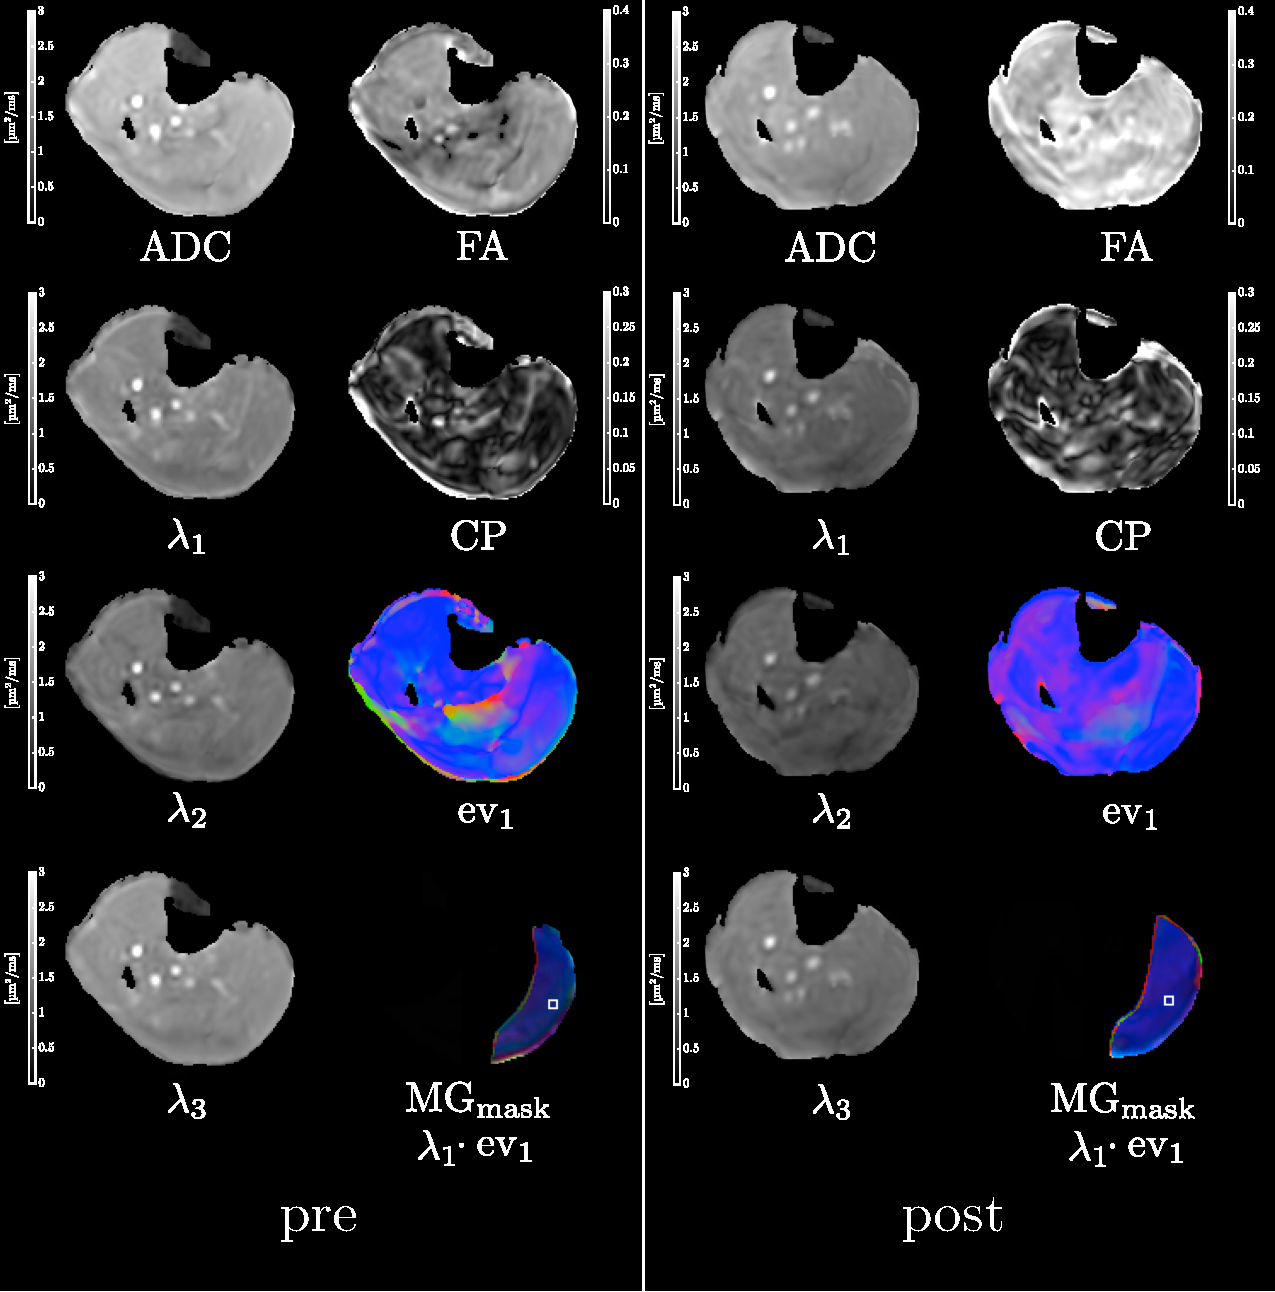
\includegraphics[width=\textwidth]{Figures/DTI_2compart.pdf}
\caption[The parametric maps extracted from the diffusion tensor]{The parametric maps extracted from the diffusion tensor.}
\label{fig: KargerEV}
\end{figure}
%*********************************************************
Visual assessment of the parametric DTI maps confirms the image quality (SNR) and lack of image artifacts (good fat suppression as well as small image distortions).
%-new paragraph-%

%-new paragraph-%
The DTI indices evaluated pre- and post-suspension in the medial gastrocnemius are summarized in Table~\ref{tab: Karger1};
the values listed here are the averages for all subjects. Three eigenvalues and apparent diffusion coefficient  decreased significantly post-suspension ($\lambda_1$:  $p = 0.025$, $\lambda_2$: $p = 0.035$, $\lambda_3$: $p = 0.049$, ADC: $p = 0.029$) while FA increased and CP decreased with suspension, although the latter indices two did not show significant changes ($p = 0.239$ for FA and $p=0.763$ for CP). 
The maximum decrease was in the secondary eigenvalue that in turn resulted in a smaller difference between the secondary and tertiary eigenvalue post suspension (reflected also as a decrease in CP).
%=========================================================
\begin{table}[!htb]
\vspace{+0.2cm}
\caption[Diffusion tensor indices pre- and post-suspension]{Diffusion tensor indices pre- and post-Unilateral Limb Suspension (ULLS).}
\label{tab: Karger1}
\begin{center}
\begin{threeparttable}
\begin{tabular}{@{}llll@{}}
\toprule[1pt]\midrule[0.3pt]
  &   & Pre-ULLS    & Post-ULLS   \\ \midrule
$\lambda_1$\tnote{$\dagger$} & $\left[\SI{}{\micro\meter^2 / \milli\second}\right]$ & 2.06 $\pm$ 0.11 & 1.91 $\pm$ 0.15 \\[6pt]
$\lambda_1$\tnote{$\dagger$} & $\left[\SI{}{\micro\meter^2 / \milli\second}\right]$ & 1.44 $\pm$ 0.08 & 1.31 $\pm$ 0.11 \\[6pt]
$\lambda_3$\tnote{$\dagger$}& $\left[\SI{}{\micro\meter^2 / \milli\second}\right]$ & 1.30 $\pm$ 0.11 & 1.17 $\pm$ 0.10 \\[6pt]
ADC\tnote{$\dagger$}   	&	& 1.60 $\pm$ 0.07 & 1.47 $\pm$ 0.11 \\[6pt]
FA   					&	& 0.25 $\pm$ 0.04 & 0.27 $\pm$ 0.04 \\ \midrule[0.3pt]\bottomrule[1pt]
\end{tabular}
\begin{tablenotes}[flushleft]\footnotesize
\item[$\dagger$] significant difference between pre- and post-suspension
\end{tablenotes}
\end{threeparttable}
\end{center}
\vspace{-0.2cm}
\end{table}
%=========================================================
In addition to the average over all subjects listed in Table~\ref{tab: Karger1}, the DTI indices (eigenvalues, ADC, FA and CP) pre- and post-suspension are also plotted for each subject individually in Figure~\ref{fig: KargerPlots}. 
This was done to confirm the consistency of DTI changes with suspension across the seven subjects and hence the validity of the data.
Pre- and post- values for each subject are connected for ease of visualization of the changes in the indices with suspension. 
For most of the DTI indices the majority of subjects show the same direction of changes: e.g., six out of seven subjects show a decrease in $\lambda_1, \lambda_2$, ADC, and an increase in FA, while five out of seven subjects show a decrease in $\lambda_3$ and in CP.
%*********************************************************
\begin{figure}[!htb]
\vspace{+0.2cm}
\centering
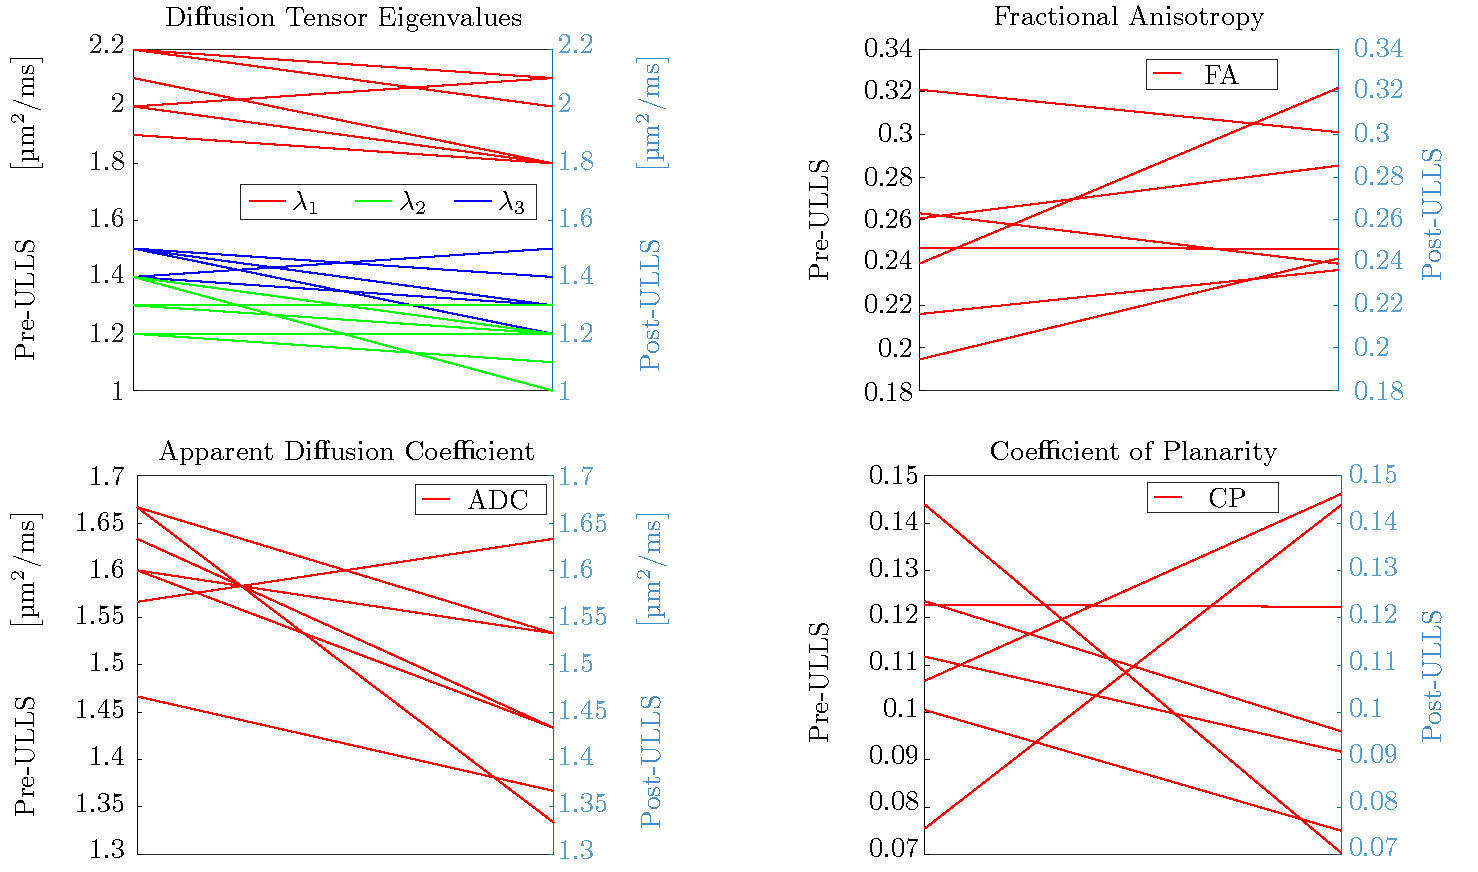
\includegraphics[width=\textwidth]{Figures/KargerPlots.pdf}
\caption[Individual plots of the DTI indices pre- and post-suspension]{Individual plots of the DTI indices pre- and post-suspension.}
\label{fig: KargerPlots}
\end{figure}
%*********************************************************
Table~\ref{tab: Karger2} lists the model parameters obtained by the search of the parameter space for the values of ($\alpha$, $d$, $\tau_{\mathrm{in}}$, $\nu_{\mathrm{in}}$, $\nu_{\mathrm{col}}$) that yielded the lowest value of the error index~\cite{RND12}. 
The increase in the ellipticity index with disuse indicates that the fiber becomes more circular, while the decrease in muscle fiber diameter is as anticipated with atrophy. 
%~~~~~~~~~~~~~~~~~~~~~~~~~~~~~~~~~~~~~~~~~~~~~~~~~~~~~~~~~
\subsection{Discussion}
%~~~~~~~~~~~~~~~~~~~~~~~~~~~~~~~~~~~~~~~~~~~~~~~~~~~~~~~~~
While it is known that the quadriceps muscles show greater atrophy than the medial gastrocnemius in aging and are a better correlate to physical function~\cite{RND27}, the motivation for the focus on the MG in the current study is based on the ease of performing functional MRI studies on the MG for correlation to structural MRI studies~\cite{RNSS4, RNCS4, Malis:2018fr, RNS16}. 
Further, calf circumference (and by extension calf muscle mass as well) has been shown in a large-scale study to provide information on muscle related disability and physical function~\cite{RND30}.
%-new paragraph-%

%-new paragraph-%
Muscle force loss was approximately greater by a factor of 3 compared to reduction in muscle mass. 
Prior work on gravitational unloading effects on fast and slow rat hind-limb muscles data indicate that predominantly slow muscles are more responsive to unloading than predominantly fast muscles~\cite{RND31}.
Since the soleus has a higher proportion of slow twitch muscles compared to the gastrocnemius muscles, it would be anticipated that the soleus would show the highest atrophy (volume decrease). 
However, comparing \% volume changes in the three muscles in the current study, larger changes were seen in the gastrocnemius muscles.  
It should be noted though that the soleus muscle had the highest changes in terms of absolute volume changes comparing pre- and post-suspension muscles.
%-new paragraph-%

%-new paragraph-%
Comparing the values of DTI indices in the current study with that reported by Karampinos~et~al.~\cite{RND12}, there are considerable differences in FA and in CP between the two studies.
The reasons for these differences may arise from differences in the measurement methodology.
A simulated echo EPI diffusion weighted sequence was used by Karampinos~et~al.~\cite{RND12} in contrast to the current study that uses a spin echo EPI diffusion weighted sequence.
It has been shown earlier that the simulated echo is better for diffusion imaging of muscle than a spin echo~\cite{RND32}. 
However, the sequence used in~\cite{RND12} has a TE of $\SI{52}{\milli\second}$~\cite{RND12} which is really long for a stimulated echo that has half the signal of a spin echo with a similar TE.
This raises the issue that the SNR of the sequence used in~\cite{RND12} may not have been high and low SNR has been shown to bias the estimation of DTI indices~\cite{RND33}.
Further, values reported for the eigenvalues and FA for the MG are in good agreement between the current study with another recent rigorous study that evaluated DTI indices for voxels with SNR $> 20$~\cite{RND33}.
%-new paragraph-%

%-new paragraph-%
Previous studies on denervation induced atrophy on rodent models showed a reduction in $\lambda_2$ and $\lambda_3$, an increase in fractional anisotropy while $\lambda_1$ was unchanged~\cite{RND8}. 
It is well accepted that DTI measurements in muscle reflect water diffusion in the intracellular space, thus the authors of this paper attributed the decrease in the secondary and tertiary eigenvalues to a decrease in the diameter of myofibers (i.e., myofiber atrophy). 
In another study, the triceps surae was assessed with DTI after Achilles tenotomy in rats~\cite{RND9}. 
Both muscle atrophy as well as a decrease in plantarflexion force was seen post-tenotomy. 
Significant decreases in $\lambda_1$, $\lambda_2$, and $\lambda_3$ and an increase in FA were seen between the control and treatment sides at four weeks post-tenotomy~\cite{RND9}. 
This is in contrast to denervation induced atrophy where no changes were seen in $\lambda_1$.
In the present study, decreases in all three eigenvalues were significant. 
The eigenvector corresponding to the lead eigenvalue is in the direction of the muscle fiber and thus $\lambda_1$ represents diffusion along the long axis of the muscle fiber. 
Since the muscle fiber is orders of magnitude greater than the diffusion distances, changes in muscle fiber length are not expected to cause changes in $\lambda_1$. 
Further, changes in fiber cross-section diameters should also not affect $\lambda_1$ as the diffusion direction is along the long axis of the muscle fiber. 
Thus, the decrease in $\lambda_1$ is difficult to explain. 
Possibly, the reduced diffusivity along the fibers' long axis is related to a loss in myosin content~\cite{RNS10} and reduction in the packing density of actin filament proteins~\cite{RND35} that result in structurally weakened sarcomeres. 
While the underlying physiological mechanisms are unclear, presented observations of a decrease in $\lambda_1$ is similar to that seen in the tenotomy induced atrophy~\cite{RND9}.
The decrease in $\lambda_2$ and $\lambda_3$ can potentially be related to a change in muscle fiber diameter and is similar to that seen in denervation induced atrophy~\cite{RND8}. 
It should also be noted that the largest decrease was seen in $\lambda_2$. 
If the secondary and tertiary eigenvalues reflect the long axis and short axis diameters respectively of the muscle fiber cross-section, then the muscle fiber is more circular post-suspension. 
%-new paragraph-%

%-new paragraph-%
In this context, Karampinos~et~al.~\cite{RND12} advanced the hypothesis that the elliptic fiber cross-section arises from a response to the mechanical stimulus as the fiber is strained more along one direction in the muscle fiber cross-section than in the orthogonal direction. 
When the mechanical stimulus is reduced or removed as with ULLS induced disuse, the preferential deformation along one axis in the fiber cross-section is removed.
This may well result in the fiber cross-section becoming more circular in the absence of a mechanical stimulus.
As opposed to the progressive circularity accompanying disuse-atrophy~\cite{RND36},
ADC decreased significantly with suspension and may potentially arise from a combination of a decrease in inherent intracellular diffusivity (decrease in all three eigenvalues) and a decrease in muscle fiber size (decrease in secondary and tertiary eigenvalues).
In the context of a reduction of a mechanical stimulus with suspension, the discussion of findings from related studies using strain/strain rate tensor imaging is worthwhile~\cite{RNSS4, RNCS4, Malis:2018fr, RNS16}. 
Strain and strain rate tensor imaging evaluate tissue deformation and the tensor provides information of the strain (or strain rate) in three orthogonal directions. 
The primary, secondary, and tertiary eigenvectors of the strain rate tensor correspond approximately to the muscle fiber direction and to two orthogonal directions in the muscle fiber cross-section, respectively. 
When the muscle fiber contracts, a negative strain will be seen along the muscle fiber direction and accompanying this, a positive strain from radial expansion will be seen in the fiber cross-section.
However, this positive strain is not symmetric in the fiber cross-section, with much larger expansion along one direction than the orthogonal direction; this asymmetry has been reported in a number of studies~\cite{Malis:2018fr, RNS16, RNS31}.
%-new paragraph-%

%-new paragraph-%
A recent study on strain rate tensor imaging after unilateral limb suspension reported that the fiber cross-section strain rate asymmetry decreased post-suspension~\cite{Malis:2018fr}.
This decrease in strain rate asymmetry may also be tied to the structural response to the lack of mechanical stimulus.
This potentially may imply that the long axis of the elliptical cross-section (proportional to the secondary eigenvalue of the diffusion tensor) is a consequence of the external mechanical stimulus since the radial expansion is preferentially along this direction resulting in an elongation of the fiber cross-section in one direction. Once this stimulus is removed (as in limb suspension) the elongated axes is no longer preferentially stretched, and may potentially become less elliptical (more circular).
This is reflected in a lower CP value post-suspension. 
Another potential explanation for the observed structural changes may be the altered muscle fiber-extracellular matrix interactions from limb suspension~\cite{RNSS4, RNCS4}. 
%-new paragraph-%

%-new paragraph-%
The values of $\alpha$ reported in the literature for the vastus lateralis muscle are in the range of $0.4$ to $0.68$~\cite{RND38, RND39}; the current value of $0.55$ for MG ellipticity in the pre-suspension case appears to be reasonable~\cite{RND38, RND39}.
Karampinos~et~al. report the value of $\alpha$ from the fit to the diffusion model with a range of $0.6 - 0.9$; the lower end of this range is close to the current paper.
The MG muscle fiber diameter extracted from the model in the current study ($\SI{82}{\micro\meter}$) is in agreement with values reported in the literature~\cite{RND38} and also with the range ($70 - \SI{110}{\micro\meter}$) determined for the MG in the earlier diffusion modeling study by Karampinos~et~al.~\cite{RND12}.
Further, the focus of the modeling was on determining if meaningful changes in microstructure with suspension can be extracted from the experimentally determined diffusion eigenvalues.
With suspension, the ratio of the short axis to long axis muscle fiber length increases which implies that the fiber becomes more circular.
In the light of the hypothesis that the elliptical muscle fiber shape arises from the mechanical stimulus, the modeling result of a more circular muscle fiber can be explained by the lack of mechanical stimulus during the 4-week suspension.
The diameter of the muscle fiber decreases; this finding is consistent with muscle fiber atrophy. 
In fitting both pre- and post-suspension DTI data, the search algorithm converged on the upper or lower limits for $\tau_{\mathrm{in}}, \nu_{\mathrm{in}}$ and $\nu_{\mathrm{col}}$.
Thus, the best-fit values for these parameters may be in error. 
The NRMSE was quite flat with respect to these variables; this was noted for $\tau_{\mathrm{in}}$ by Karampinos~et~al.~\cite{RND12}, and thus, fitting the available DTI data to this model does not allow one to draw conclusions regarding $\tau_{\mathrm{in}}, \nu_{\mathrm{in}}$ and $\nu_{\mathrm{col}}$.
%-new paragraph-%

%-new paragraph-%
There are limitations to the current study: the study population is small but since it is a longitudinal study (pre- and post-ULLS), statistical significance was reached for the changes in the eigenvalues. 
A one-point diffusion measurement is not ideal for extracting tissue parameters through modeling; future work using multi-point DTI data (obtained for example, by varying diffusion time and/or \mbox{\textit{b-}value}s) will allow more robust modeling to extract accurate values for these microstructural features. 
Further, multi-point DTI data may allow greater flexibility to extend to single subject rather than limit to cohort modeling as in the current study.
It should also be noted that if the fit was performed independently on each subject, it would have allowed testing of the significant changes in the microstructural parameters with limb suspension.
Measurements on the contralateral leg would have provided information on the effects of a change in mechanical loading of the unsuspended leg.
However, the current study was part of a larger protocol that besides DTI, included quantification of fat, connective tissue as well as functional measurements and acquiring data on the contralateral leg would have prolonged the scanning time excessively.
Further, imaging both legs at the same time was restricted by the customized coil that accommodated only one leg.
However, the customized coil provided higher SNR than vendor coils and allowed the acquisition of the entire lower leg without repositioning the subject.
%~~~~~~~~~~~~~~~~~~~~~~~~~~~~~~~~~~~~~~~~~~~~~~~~~~~~~~~~~
\subsection{Conclusion}
%~~~~~~~~~~~~~~~~~~~~~~~~~~~~~~~~~~~~~~~~~~~~~~~~~~~~~~~~~
The current study shows that the DTI eigenvalues decrease with suspension induced disuse atrophy. 
Experimentally, the secondary eigenvalue showed the largest decrease with suspension.
This could potentially be related to a hypothesis that attributes the elliptical shape of the muscle fiber cross-section as arising from a response to an external load~\cite{RND12}. 
While it is still a conjecture, the asymmetry of deformation in the fiber cross-section may result in one axis becoming longer than the orthogonal one and then unloading conditions can cause this shape asymmetry to be reduced. 
As the secondary and tertiary eigenvalues are related to the fiber cross-section diameters, this results in larger changes in the secondary eigenvalue as the fiber reduces the most in diameter along this direction with unloading. 
An exploratory modeling of the DTI data to extract microstructural parameters showed that it is feasible and the disuse atrophy related changes in muscle ellipticity, mean diameter, residence time, intracellular volume and collagen volume extracted from the model were physiologically reasonable.
%=========================================================
\section{Random Permeable Barrier Modeling of Age Induced Changes in the Time Dependent Diffusion Eigenvalues}
\label{sec: STEAM RPBM}
%=========================================================
Muscle mass loss have been reported in the aging muscle and this is in part, responsible for functional loss. 
However, non-invasive monitoring of microstructural changes as in muscle fiber diameter with age has not been reported. 
Commonly employed diffusion weighted acquisition protocols collect data at a single diffusion time. 
The time dependence of the diffusion tensor eigenvalues can provide additional information to improve quantification of tissue microstructure. 
A diffusion model is required to make inferences about the microstructure from the time dependent eigenvalue data.
Random permeability barrier model (RPBM) was recently introduced and applied to retrieve microscopic parameters such as membrane permeability and fiber diameter in human skeletal muscles~\cite{NovikovRPBM, RND13}. 
%~~~~~~~~~~~~~~~~~~~~~~~~~~~~~~~~~~~~~~~~~~~~~~~~~~~~~~~~~
\subsection{Random Permeable Barrier Model}
%~~~~~~~~~~~~~~~~~~~~~~~~~~~~~~~~~~~~~~~~~~~~~~~~~~~~~~~~~
The model treats muscle as a volume with randomly oriented infinite flat semipermeable membranes. 
For each membrane permeability ($\kappa$) relates the difference in concentrations on both sides of the membrane and the flux through it which provides the following boundary conditions:
%.........................................................
\begin{equation}\label{eq: RPBM bc}
D_0\mathbf{n}\left.\frac{\partial{c}}{\partial r} \right\vert_{\pm} = \kappa \left[ c|_+ - c|_-  \right]
\end{equation}
%.........................................................
RPBM model is characterized by three parameters: the free diffusion coefficient ($D_0$), membrane surface to volume ratio ($S/V$) and permeability ($\kappa$). Time-dependent diffusion coefficient is found by solving the diffusion equation (Equation~\ref{eq:Fick2}) and then averaging the result over disorder using real-space renormalization group~\cite{NovikovRPBM}.
%.........................................................
\begin{equation}\label{eq: RPBM}
D(t) = \frac{D_0}{2\pi t}\int\limits^{\infty}_{-\infty}\dfrac{d\omega}{(-i\omega)^2}\frac{e^{-i\omega t}}{1 + \zeta +2z_{\omega}(1-z_{\omega})  \left[\sqrt{1+\zeta/\left(1-z_{\omega}\right)}-1 \right] }
\end{equation}
%.........................................................
where $z_\omega = i \sqrt{i \omega t}$ and $\zeta=(S/V)D_0/4\kappa$ is an effective volume fraction occupied by membranes.
The integral~(\ref{eq: RPBM bc}) can be integrated numerically as outlined in reference~\cite{RND13}.
%~~~~~~~~~~~~~~~~~~~~~~~~~~~~~~~~~~~~~~~~~~~~~~~~~~~~~~~~~
\subsection{Materials and Methods}
%~~~~~~~~~~~~~~~~~~~~~~~~~~~~~~~~~~~~~~~~~~~~~~~~~~~~~~~~~
Image acquisition protocol used a custom-built STEAM-EPI DTI sequence (Figure~\ref{fig: STEAM_GE}) discussed in more details in section~\ref{sec: EPI}. 
A water selective SPSP RF-pulse was used for fat suppression. 
Six non-collinear gradient directions with a nominal \mbox{\textit{b-}value} of $\SI{400}{\second \per\milli\meter^2}$ were used to map the direction dependent diffusion at ten values of the diffusion time~$\Delta$ ($\SI{20}{\milli\second}$ to $\SI{600}{\milli\second}$). 
Imaging parameters were: echo time (TE) $\SI{32}{\milli\second}$, repetition time (TR) $\SI{4000}{\milli\second}$, $2$ signal averages, acquisition matrix size $80 \times 80$, field of view (FOV) $200 \times 200 \; \SI{}{\milli\meter^2}$, 3 slices of $\SI{5}{\milli\meter}$ thickness. 
Diffusion data were pre-processed for eddy current mis-registration and denoised by applying Joint-Rican LMMSE filter~\cite{RND24} prior to computing the diffusion tensor and the diffusion eigenvalues. 
The corrected full \textit{b-}matrix that accounted for the diffusion, imaging and crusher gradients was calculated as outlined in subsection~\ref{subsection: STEAM b value}. For the nominal $b = 0$ images, the \mbox{\textit{b-}value} varied from $\SI{1.7}{\second \per  \milli\meter^2}$ at $\Delta = \SI{20}{\milli\second}$ to $\SI{22}{\second\per\milli\meter^2}$ at $\Delta = \SI{600}{\milli\second}$ and for the nominal $b = \SI{400}{\second\per\milli\meter^2}$ images, the \mbox{\textit{b-}value} varied from $\SI{371}{\second\per\milli\meter^2}$ at $\Delta = \SI{20}{\milli\second}$ to $\SI{547}{\second\per\milli\meter^2}$ at $\SI{600}{\milli\second}$, emphasizing the need for full \textit{b-}matrix calculation. 
Prior to human scans a set of images was obtained in a water phantom following the same imaging protocol as described above. 
Fractional anisotropy (FA) maps were calculated from the acquired data to validate diffusion tensor calculations at long diffusion times. 
FA maps side by side with the corresponding magnitude images at nominal \mbox{\textit{b-}value} for diffusion times 20 and $\SI{600}{\milli\second}$ are show in the Figure~\ref{fig:STEAM phantom}. 
%*********************************************************
\begin{figure}[!htb]
\vspace{+0.2cm}
\centering
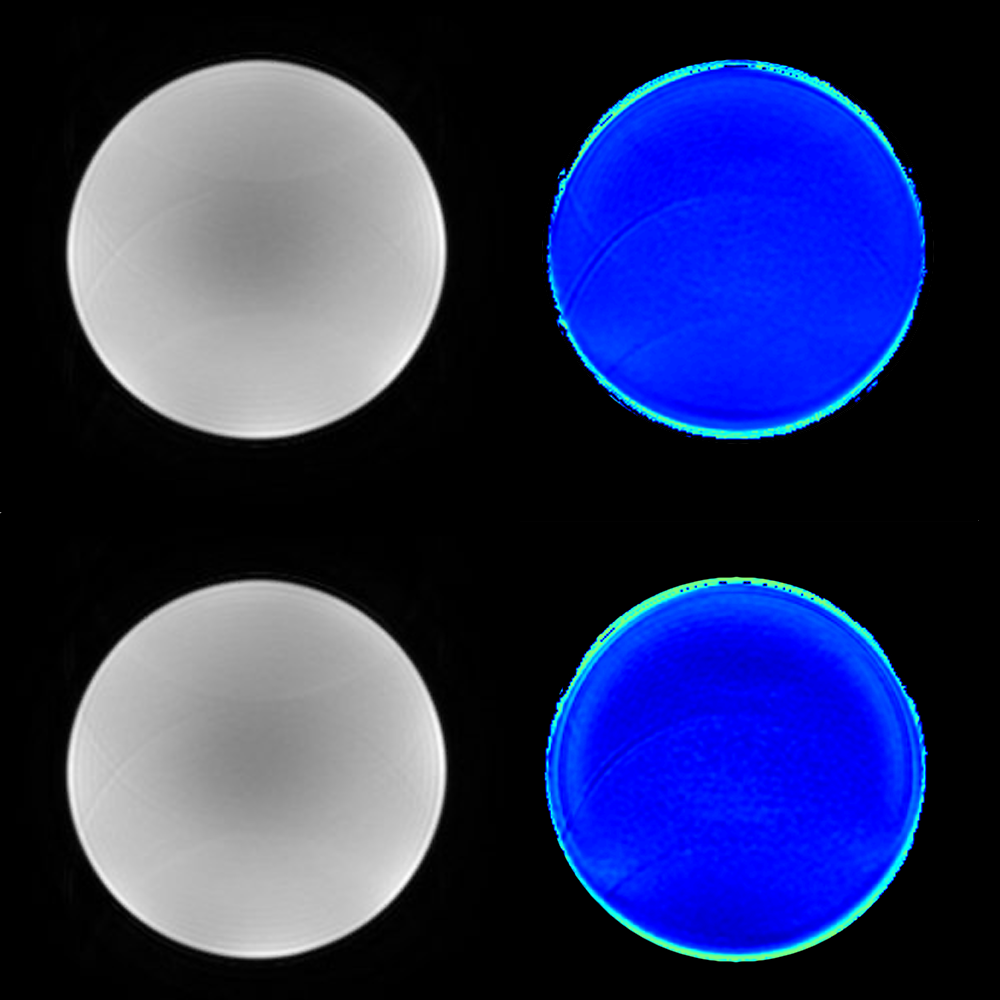
\includegraphics[width=0.9\textwidth]{Figures/STEAM_Phantom.pdf}
\caption[Baseline magnitude images and FA colormaps of water phantom acquired with STEAM-EPI DTI image sequence at two diffusion times]{Baseline magnitude images and FA colormaps of water phantom acquired with STEAM-EPI DTI image sequence at two mixing times: 20 and $\SI{590}{\milli\second}$.}
\label{fig:STEAM phantom}
\end{figure}
%*********************************************************
%-new paragraph-%

%-new paragraph-%
All human imaging studies were performed after IRB approval on a $\SI{3}{\tesla}$ scanner (GE Medical Systems, WI, USA) on seven young ($31 \pm 8$ years) and six senior ($75 \pm 5$ years) subjects. 
The RPBM model was fitted by fixing the free diffusion coefficient $D_0$ at the long diffusion time limit of the primary eigenvalue ($\lambda_1$) to extract the following parameters: the membrane permeability ($\kappa$), and the membrane surface to volume ratio ($S/V$). 
The myofiber size (a) is derived from the surface to volume ratio as: $4V/S$. 
The RPBM fits were made to the time dependence of the average of $\lambda_2$, and $\lambda_3$ ($D_{\perp}$); the values of $D_{\perp}$ were the average over the medial gastrocnemius (MG) muscle segmented from all three~slices.
%~~~~~~~~~~~~~~~~~~~~~~~~~~~~~~~~~~~~~~~~~~~~~~~~~~~~~~~~~
\subsection{Results}
%~~~~~~~~~~~~~~~~~~~~~~~~~~~~~~~~~~~~~~~~~~~~~~~~~~~~~~~~~
Figure~\ref{fig:STEAM_EV} shows parametric $D_\parallel$ and $D_\perp$ maps for a young and for a senior subject at two diffusion times.
Excellent fat suppression was seen in all the STEAM DTI data. 
Typical eigenvalue images ($D_\parallel \equiv \lambda_1$) and ($D_\perp \equiv (\lambda_2 + \lambda_3)/2$) at two values of mixing time ($20$ and $\SI{590}{\milli\second}$) for a young (left panel) and a senior (right panel) subject. 
The decrease in SNR with diffusion time can be visualized by the noisier images of the bottom panel. 
%*********************************************************
\begin{figure}[!htb]
\vspace{+0.2cm}
\centering
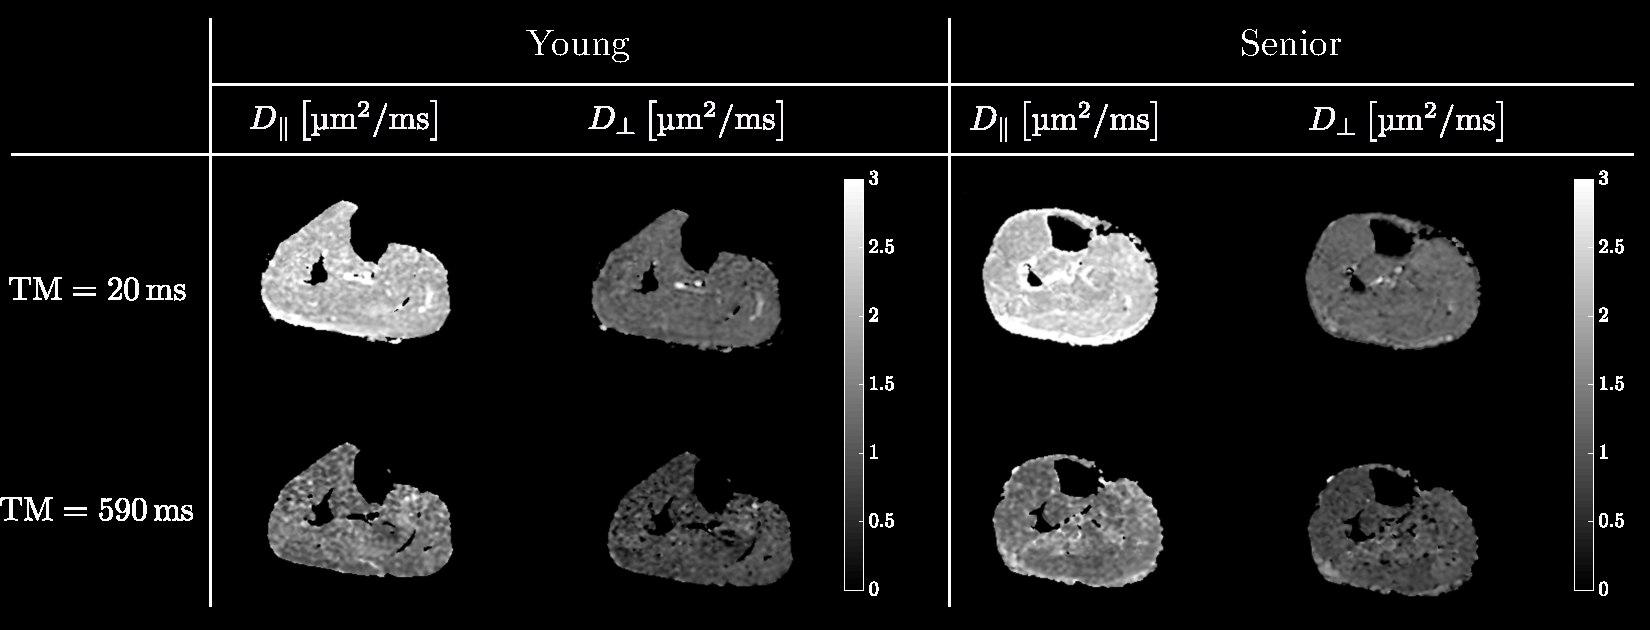
\includegraphics[width=0.9\textwidth]{Figures/STEAM_EV.pdf}
\caption[Diffusion tensor eigenvalues grayscale maps at two values of mixing time  for a young and a senior subject]{Diffusion tensor eigenvalues $D_\parallel$ and $D_\perp$ grayscale maps at two values of mixing time (20 and $\SI{600}{\milli\second}$) for a young (left) and a senior (right) subject. The decrease in SNR with TM can be visualized by the noisier images of the bottom panel.}
\label{fig:STEAM_EV}
\end{figure}
%*********************************************************
%=========================================================
\begin{table}[!htb]
\vspace{+0.2cm}
\begin{center}
\caption[Diffusion eigenvalues at different mixing times]{Diffusion eigenvalues ($\lambda_1, \lambda_2, \lambda_3$) at different mixing times.}
\label{tab:RPBM}
\begin{tabular}{@{}ccccccccc@{}}
\toprule[1pt]\midrule[0.3pt]
\multirow{2}{*}{$\mathrm{TM}$ {[}ms{]}} & \multicolumn{2}{c}{$\lambda_1 \quad [\SI{}{\micro\meter^2\per\milli\second}]$}  &  & \multicolumn{2}{c}{$\lambda_2 \quad [\SI{}{\micro\meter^2\per\milli\second}]$}  &  & \multicolumn{2}{c}{$\lambda_3 \quad [\SI{}{\micro\meter^2\per\milli\second}]$}  \\ \cmidrule(lr){2-3} \cmidrule(lr){5-6} \cmidrule(lr){8-9} 
                             & Young     & Senior    &  & Young     & Senior    &  & Young     & Senior    \\ \cmidrule(){1-9}
20                           & 2.8 $\pm$ 0.2 & 2.8 $\pm$ 0.2 &  & 2.4 $\pm$ 0.1 & 2.3 $\pm$ 0.3 &  & 1.2 $\pm$ 0.1 & 1.2 $\pm$ 0.1 \\
30                           & 2.6 $\pm$ 0.2 & 2.7 $\pm$ 0.2 &  & 2.0 $\pm$ 0.1 & 2.1 $\pm$ 0.3 &  & 1.2 $\pm$ 0.1 & 1.3 $\pm$ 0.1 \\
60                           & 2.4 $\pm$ 0.2 & 2.5 $\pm$ 0.2 &  & 1.9 $\pm$ 0.2 & 1.8 $\pm$ 0.2 &  & 0.8 $\pm$ 0.1 & 1.0 $\pm$ 0.2 \\
90                           & 2.4 $\pm$ 0.3 & 2.4 $\pm$ 0.2 &  & 1.7 $\pm$ 0.2 & 1.7 $\pm$ 0.2 &  & 0.8 $\pm$ 0.1 & 0.9 $\pm$ 0.1 \\
190                          & 2.3 $\pm$ 0.3 & 2.3 $\pm$ 0.2 &  & 1.7 $\pm$ 0.1 & 1.7 $\pm$ 0.2 &  & 0.4 $\pm$ 0.1 & 0.6 $\pm$ 0.1 \\
290                          & 2.2 $\pm$ 0.2 & 2.2 $\pm$ 0.2 &  & 1.8 $\pm$ 0.1 & 1.7 $\pm$ 0.1 &  & 0.2 $\pm$ 0.1 & 0.4 $\pm$ 0.1 \\
340                          & 2.2 $\pm$ 0.1 & 2.2 $\pm$ 0.2 &  & 1.2 $\pm$ 0.1 & 1.3 $\pm$ 0.1 &  & 0.7 $\pm$ 0.1 & 0.8 $\pm$ 0.1 \\
390                          & 2.2 $\pm$ 0.1 & 2.2 $\pm$ 0.3 &  & 1.3 $\pm$ 0.2 & 1.3 $\pm$ 0.2 &  & 0.7 $\pm$ 0.1 & 0.7 $\pm$ 0.1 \\
490                          & 2.1 $\pm$ 0.1 & 2.2 $\pm$ 0.2 &  & 1.3 $\pm$ 0.2 & 1.3 $\pm$ 0.1 &  & 0.6 $\pm$ 0.1 & 0.7 $\pm$ 0.1 \\
590                          & 2.1 $\pm$ 0.2 & 2.2 $\pm$ 0.2 &  & 1.3 $\pm$ 0.2 & 1.3 $\pm$ 0.1 &  & 0.6 $\pm$ 0.1 & 0.7 $\pm$ 0.1 \\ \midrule[0.3pt]\bottomrule[1pt]
\end{tabular}
\end{center}
\vspace{-0.2cm}
\end{table}
%=========================================================
Table~\ref{tab:RPBM} summarizes the eigenvalues for the MG muscle in the young and senior cohort at the ten diffusion times. 
Larger changes with diffusion time are seen in $\lambda_2$, and $\lambda_3$ (compared~to~$\lambda_1$). 
The RPBM fits to the time dependence of $D_\perp$ for a subject from the young cohort and from the senior cohort are shown for the Figure~\ref{fig:RPBM fit}. The large variation of $D_\perp$ with TM is in contrast to the smaller variation of $D_\parallel$ with TM.
Table~\ref{tab:RPBM2} is a list of model derived muscle microstructure parameters; volume fraction decreased with age while diffusion time and residence time in a cell increased with age while other model parameters such as the fiber size and membrane permeability increased with age but did not reach significance.
%*********************************************************
\begin{figure}[!htb]
\vspace{+0.2cm}
\centering
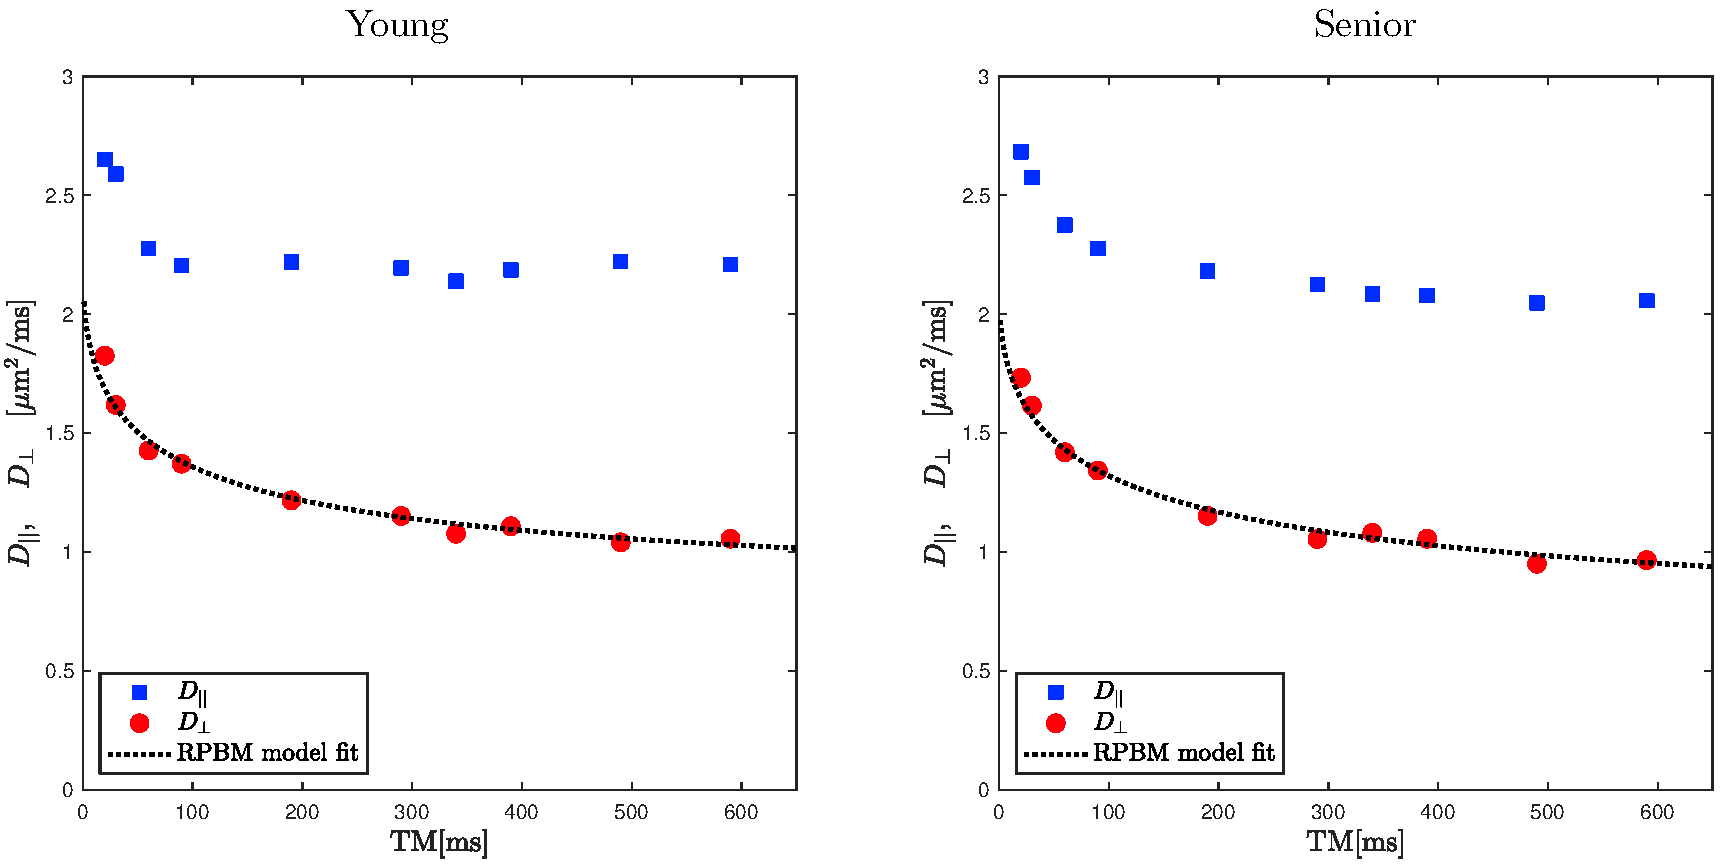
\includegraphics[width=\textwidth]{Figures/RPBM_fit.pdf}
\caption[RPBM model fit to the time dependence of diffusion indices for a young and senior subjects]{RPBM model fit to the time dependence of diffusion indices for a young and senior subjects.}
\label{fig:RPBM fit}
\end{figure}
%*********************************************************
%=========================================================
\begin{table}[!htb]
\vspace{+0.2cm}
\begin{center}
\caption[Parameters of muscle tissue extracted from the RPBM model]{Parameters of muscle tissue extracted from the RPBM model.}
\label{tab:RPBM2}
\begin{tabular}{@{}lrr@{}}
\toprule[1pt]\midrule[0.3pt]
                        								& \multicolumn{1}{c}{Young}         & \multicolumn{1}{c}{Senior}  \\ \cmidrule(){1-3}
$D_0 \; \left[\SI{}{\micro\meter^2\per\milli\second}\right]$      & \multirow{2}{*}{2.20 $\pm$ 0.16}  & \multirow{2}{*}{2.18 $\pm$ 0.24}   \\
free diffusion          								&                                	&                                \\[6pt]
$\zeta$                 								& \multirow{2}{*}{3.26 $\pm$ 1.62}  & \multirow{2}{*}{2.79 $\pm$ 0.63}   \\
volume fraction         								&                                	&                                 \\[6pt]
$S/V \; \left[\SI{}{\micro\meter^{-1}}\right]$                      & \multirow{2}{*}{0.14 $\pm$ 0.03}  & \multirow{2}{*}{0.13 $\pm$ 0.02}   \\
surface to volume ratio 								&                                	&                                 \\[6pt]
$\kappa \; \left[\SI{}{\micro\meter / \milli\second}\right]$		& \multirow{2}{*}{0.025 $\pm$ 0.005}& \multirow{2}{*}{0.027 $\pm$ 0.009} \\
permeability            								&                                	&                                 \\[6pt]
$a \; \left[\SI{}{\micro\meter}\right]$                        	& \multirow{2}{*}{28.63 $\pm$ 4.94} & \multirow{2}{*}{32.00 $\pm$ 3.72}  \\
myofiber diameter       								&                                	&                                 \\[6pt]
$\tau_{R} \; \left[\SI{}{\milli\second}\right]$                        								& \multirow{2}{*}{552.2 $\pm$ 122.1}& \multirow{2}{*}{650.6 $\pm$ 159.2} \\
residence time  								&                                	&                                 \\[6pt]
$\tau_{D} \; \left[\SI{}{\milli\second}\right]$                       								& \multirow{2}{*}{194.5 $\pm$ 71.9} & \multirow{2}{*}{238.1 $\pm$ 50.7}  \\
diffusion time  								&                                	&                                \\ \midrule[0.3pt]\bottomrule[1pt]
\end{tabular}
\end{center}
\vspace{-0.2cm}
\end{table}
%=========================================================
%~~~~~~~~~~~~~~~~~~~~~~~~~~~~~~~~~~~~~~~~~~~~~~~~~~~~~~~~~
\subsection{Discussion} 
%~~~~~~~~~~~~~~~~~~~~~~~~~~~~~~~~~~~~~~~~~~~~~~~~~~~~~~~~~
The values of the model derived parameters are in general agreement with that reported for the MG in an earlier study. 
The RPBM model yields a lower volume fraction for the aging muscle which is a measure of the membrane's ability to hinder diffusion. 
It is possible that aging muscle may have compromised sarcolemma integrity that makes it more permeable and thus poses less of a barrier to diffusion. 
Based on the fact that muscle atrophies with age a decrease in fiber diameter with age is expected. 
However fiber diameters derived from the RPBM model did not show anticipated changes. 
A sarcolemma with compromised integrity (as seen here in aging muscle) may potentially affect lateral transmission of force, the latter is mediated by proteins in the sarcolemma.
%~~~~~~~~~~~~~~~~~~~~~~~~~~~~~~~~~~~~~~~~~~~~~~~~~~~~~~~~~
\subsection{Conclusions} 
%~~~~~~~~~~~~~~~~~~~~~~~~~~~~~~~~~~~~~~~~~~~~~~~~~~~~~~~~~
The study has demonstrated the potential of diffusion modeling to extract muscle tissue parameters from time dependent $D_\perp$ derived from DTI data and its potential application it to study age related skeletal muscle remodeling.
%~~~~~~~~~~~~~~~~~~~~~~~~~~~~~~~~~~~~~~~~~~~~~~~~~~~~~~~~~
\section{Acknowledgments}
%~~~~~~~~~~~~~~~~~~~~~~~~~~~~~~~~~~~~~~~~~~~~~~~~~~~~~~~~~
Section~\ref{sec: DTI ULLS} is a reprint of material, with additional details provided in subsection~\ref{subsec: bicompart}, as it appears in: V.~Malis, U.~Sinha, R.~Csapo, M.~Narici, E.~Smitaman, and S.~Sinha, ``Diffusion tensor imaging and diffusion modeling: Application to monitoring changes in the medial gastrocnemius in disuse atrophy induced by unilateral limb suspension,'' \emph{J. Magn. Reson. Imaging}, vol. 49, no. 6, pp. 1655-1664, Dec. 2018.
The author of the dissertation was the primary author of this paper.
%-new paragraph-%

%-new paragraph-%
Section~\ref{sec: STEAM RPBM} is a reprint of material, with additional details, as it appears in: V.~Malis, S.~Sinha, E.~Smitaman, and U.~Sinha, ``Skeletal Muscle Diffusion Modeling to Identify Age Related Remodeling of Muscle Microstructure,'' \emph{Proceedings of the International Society of Magnetic Resonance in Medicine}, Sydney, 2020.
The author of the dissertation was the primary author of this abstract.